%************************************************
\chapter{Similarity Search}\label{ch:cost}
%************************************************
\section{The cost of similarity search}
Having established the link between JSD and SED, we should now like to compare them.  Since both give the same ordering, we must examine efficiency.  We will compare them using intrinsic dimensionality (IDIM) and a probabilistic analysis designed to measure the cost and general notion of the tractability of similarity search techniques over high-dimensional metric spaces.  

Intrinsic dimensionality has been introduced as a tractability measure\cite{}, and a lower bound for index cost has been established. In practice, however, we have found different approximately-Gaussian distance distributions with the same IDIM may have very different probability densities close to the origin, and this has a far greater implication on performance than the IDIM. IDIM is really meaningful only within the context of a close-to-perfect Gaussian distribution, to which many metric/data combinations do not conform.

To address these limitations, we have constructed a methodology to perform a probabilistic analysis over metric spaces. Like IDIM, it is based
only on the distances over data, rather than the data itself. According to probability densities at both the median, and close to the origin. We show how this can be used to estimate the cost of a search operation over a given size of data.  It can be calculated via random sampling over a data set, and we have assessed performance predictions against measured performances on various data sets and found to be useful.

Many metric spaces over which similarity search is desirable suffer from the so-called curse of dimensionality. In the domain of Similarity Search, this refers to the effect whereby, as the number of dimensions increases, the distance between any two arbitrarily selected points is increasingly less likely to be relatively either small or large, and ever more distances become close to the median. As most measured distances become closer, any indexing mechanism becomes less effective.

As similarity search matures, ever more data collections and distance metrics become subject to these techniques; the question of whether a given combination of data and metric is likely to lead to tractable searching is therefore an important one.

Much research into the cost of search-based query is in the domain of complexity analysis, and does not take dimensionality into account. Our approach is more akin to abstract interpretation, with the intent of giving a realistic measurement of efficacy which can take into account issues such as the data size, the semantic effectiveness of the metric, and the query threshold chosen as an implication of these. Although independent of any particular indexing mechanism, the resulting measurement does seem to give a good indication of realistic query cost as measured against a number of different index structures.

In outline, our method for performing an estimate of effectiveness comprises:
\begin{itemize}
\item First, a probability density function $f(x)$ for the metric space $M = (X, d)$  is established by the repeated application of $d$ over object pairs randomly sampled from $X$;
\item Using $f$, the magnitude of the collection $|X|$, and the semantic accuracy of the metric $d$, a likely query threshold $t$ is determined;
\item Using $f$ and $t$, the probability $p$ of a successful pivot operation around the median distance is established;
\item Using $|X|$ and $p$, a pragmatic upper bound of the likely number of distance calculations required at query time is established.
\end{itemize}
We will then show with a number of different datasets which distance metrics have the lowest upper bound cost for searching using a typical metric index.
\subsection{Indexing, pivoting and probabilities}
The majority of metric space indexing techniques rely upon the notion of pivoting, which in turn relies upon the triangle inequality property of the metric in question. To understand how well a given metric and data collection will perform, it is necessary to understand the probability of an indexing mechanism performing a successful prune of the search space at each step.

With respect to a pivot object p, a query object q, a query radius $r$, a pivot covering radius $\mu$:
\begin{itemize}
\item if $d(p,q) - r > \mu$, then those points known to be within $\mu$ of $p$ cannot be within $r$ of $q$
\item if $d(p,q) + r \leq \mu$, then those points known to be outside $\mu$ of $p$ cannot be within $r$ of $q$
\end{itemize}

The efficacy of any index structure built using these principles depend upon the probability of each of these two events. These probabilities are defined here as $p(e)$, the exclusion probability, and $p(i)$, the inclusion probability, respectively. From the structure of their definitions it is clear that both events are mutually exclusive, and so the probability of either one occurring can be expressed as $p(e) + p(i)$. Further, this sum is $\leq$ 1, with the sum being 1 if and only if $r = 0$; thus, if the search is for the query object itself, or those within the same equivalence class, then the pivoting mechanism turns into a deterministic fetch. More commonly $r$ will not be $0$, in which case it is clear that smaller it is, the closer $p(e) + p(i)$ will be to 1, giving better query performance.

\subsection{Probability density functions and pivoting}
Probability density functions are mathematically quite different from histograms; a very good approximation to a pdf, however, can be obtained experimentally by constructing a fine-granularity histogram over a large number of sample measurements, dividing each count by the total number of measurements over the granularity of the histogram, and using interpolation to treat the outcome as a continuous function. 

With respect to a probability density function $f(x)$ of a given distance metric over a data collection, the exclusion probability $p(e)$ can be quantified as:
\begin{equation}
	p(e) = \int_{\mu + r}^1 f(x)
\end{equation}
and similarly the inclusion probability:
\begin{equation}
	p(i) = \int_0^{\mu - r} f(x)
\end{equation}
As $\int_0^1 f(x) = 1$ and the exclusion and inclusion events are mutually exclusive, the probability of either occurring is
\begin{equation}
	p(e) + p(i) = 1 - \int_{\mu - r}^{\mu + r} f(x)
\end{equation}
If the covering radius $\mu$ is chosen to be the median, this probability represents the likelihood of excluding half of the objects covered by that pivot.

For a distance function and data collection whose pdf approximates to Gaussian, this probability depends only on the standard deviation and query threshold; it is worth noting that it is independent of the actual value of the median, and therefore to a degree independent of the IDIM.
It is very likely that the IDIM will be strongly related to the requirement for a given query threshold, a greater IDIM usually implying a greater threshold. It is, however, clear that the query threshold is the predominant factor with respect to the performance of any mechanism relying upon these probabilities.

\subsection{Query thresholds and PDFs}
While a Gaussian distribution is often a very good overall approximation for the probability of distance for a pair of random points drawn from a large space, it is never a good approximation for small distances. The reason is that Gaussian distributions are defined in the range $-\infty$ to $\infty$, but the outcome of a distance metric always has a probability of zero for values less than zero.

This distinction is important; even metrics that show very close correlation with Gaussian distributions across most of the range show markedly different behaviours close to the origin. A threshold distance for a large data collection for example may well be set so that one-millionth of the data is likely to be returned; that threshold may vary widely with different metrics that have the same median and standard deviation, and the Gaussian model is likely to place it to the left of the origin.

%\subsection{Fractions and Thresholds}
%The left hand graph in Figure 3 gives a good indication of where a threshold would need to be set in order to extract a given fraction of the data. For example, with a data set of 10 9 objects, conforming to these probabilities, the threshold 0.034 is required to fetch an average of 1000 neighbours for metric A, and a threshold of 0.0051 is required for the other metrics.
%These figures can now be used to quantify Equation 1, giving the probabilities shown in Table 1 for a successful prune at each pivot check. As a general rule, an outcome of much greater than 0.5 is likely to lead to quite successful indexing performance, and one of much less than 0.5 is likely to lead to quite bad indexing performance. While it can be seen that the outcomes given here do correspond with IDIM, they also give a much finer-grained insight into the likely performance at different thresholds. To show that the correspondence with IDIM is not always close we also include figures for another metric D 4 , which can be seen to have a higher IDIM than A but gives significantly better predicted outcomes.
%In Section 4, we further quantify how these probabilities are likely to translate into performance of an index structure.

For analysis, we consider a balanced Vantage Point Tree structure constructed around the median distance of the metric space.
A Vantage Point tree over the metric space $M = (X, d)$ is a binary tree where each node holds a single element of $X$. For every node holding a point $x_i$ , every node (if any) within the left-hand subtree contains a point $x_j$ such that $d(x_i, x_j) < \mu$  (where $\mu$ is the median of the range of $d$ over $X$), and every node within the right-hand subtree contains a point $x_j$ such that $d(x_i , x_j ) > \mu$.

A VP-tree can be created by the following algorithm:
\begin{itemize}
\item A point added to an empty tree results in a single node containing that point.
\item A point $x_j$ added to an existing node containing point $x_i$ at its head results in a new tree with that point added to the left branch if $d(x_i, x_j) < \mu$, and with that point added to the right branch otherwise.
\end{itemize}

A VP-tree for collection $X$ is then constructed by taking all the points of $X$ in an arbitrary order and adding them to an empty tree.
To allow analysis, we make the following assumptions:
\begin{itemize}
\item The tree is perfectly balanced, i.e. the size of $X$ is $2n - 1$, for some n, and every branch from root to leaf is the same length.
\item Every node of the tree is constructed with respect to the same pivot value 
\item No further mechanism or strategy exists to optimise the tree or its indexing.
\item For any three arbitrarily selected objects $x_i, x_j$ and $x_k$, then $d(x_i, x_j), d(x_j, x_k)$ and $d(x_i, x_k)$ are all probabilistically independent of each other.
\end{itemize}

Given the probabilities $p(e)$ and $p(i)$ defined above, and a perfectly-behaved Vantage Point Tree, it is possible to derive a cost estimate for querying data collections of different sizes.

\subsection{Number of distance calculations}
The method of construction of the tree in conjunction with the triangle inequality property of allows the search space to be pruned in the manner given. To consider the quantification of this process, we consider the complements of the exclusion and inclusion probabilities defined above, $q(e)$ and $q(i)$, representing respectively the probability that the left and right subtrees will be visited by the search algorithm.

Now consider the probability of visiting each node in the tree. The probability of visiting the root node is 1, that of the left hand subtree is $q(e)$ and that of the right hand subtree is $q(i)$. More generally, for any node $n$, if the probability of visiting node N is $p(n)$, then the probability of visiting its left subtree is $p(n)q(e)$ and that of visiting its right subtree is $p(n)q(i)$.
For the four nodes at level 2 of the tree, considered from left to right, the probability of visiting each is therefore: $q(e)^2$, $q(e)q(i)$, $q(i)q(e)$ and $q(i)^2$ respectively. Over many uses of this tree to perform a search, it is therefore the case that the mean number of nodes visited at this level will be 
\begin{equation}
q(e)^2 + 2q(e)q(i) + q(i)^2
\end{equation}

At the third level of the tree this mean figure is 
\begin{equation}
q(e)^3 + 3q(e)^2q(i) +3q(e)q(i)^2 + q(i)^3
\end{equation}
It can be seen that these sums respectively represent $(q(e) + q(i))^2$  and $(q(e) + q(i))^3$.

By induction over the tree structure, the mean number of nodes to be visited at depth d is $(q(e) + q(i))^d$, and for a perfectly balanced tree of depth $d$ the mean number of nodes to be visited for a whole traversal is therefore
\begin{equation}
	\sum_{i=0}^d (q(e) + q(i))^i
\end{equation}
which can now be written succinctly as a function over a metric space $M = (X, d)$:
Let $f(x)$ be the probability density function of $d$ over $X$, with median $\mu$;  let $h$ be the height of a perfectly balanced VP tree containing $X$. Then for a query threshold $r$, let the query cost estimator C be defined as

\begin{align}
	C & = \sum_{i = 0}^h (q(e) + q(i))^i\\
	  & = \frac{(q(e) + q(i))^{h+1} - 1}{q(e) + q(i) - 1}\\
	  & = \frac{\left( \int_0^{\mu+r} f(x) + \int_{\mu - r}^1 f(x) \right)^{h+1} - 1}{\left( \int_0^{\mu+r} f(x) + \int_{\mu - r}^1 f(x) \right) - 1}\\	  
	  & = \frac{\left(1 + \int_{\mu - r}^{\mu+r} f(x)  \right)^{h+1} - 1}{\int_{\mu - r}^{\mu+r} f(x)}
\end{align}
The importance of the effect of $r$ on the calculation is clearly highlighted, given that $h$ is likely to be in the region of 20 - 30 for many applications of similarity search.

For a space with $n$ nodes the maximum height $h$ of a binary tree is $\log_2(n + 1) - 1$. 
\section{Comparison of distance metrics}
A central requirement of metric space indexing structures is that the distance metric has the triangle inequality property. In their definitional form none of NCD, CPD, SED nor Jensen-Shannon divergence obeys triangle inequality, and are thus not proper distance metrics. 
% Using the method of extracting paths from trees described above, however, leads to vectors that do not exhibit the pathological cases violating triangle inequality for SED; 
Raising SED to the power of 0.48 achieves triangle inequality for vectors not generated in this manner.  Recently, \cite{} have shown that the square root of Jensen-Shannon divergence is also a proper metric.  We know of no transformation to NCD or CPD to allow their use in a metric space indexing structure and thus exclude them from the following comparison.

We applied the cost function described above on both generated and real-world data to compare the techniques described in this chapter.

%\ToDo{Run these experiments}
%
\begin{table}[h]
  \centering
\begin{tabular*}{\textwidth}{l @{\extracolsep{\fill}}rlrrrrrr}
\toprule
			    &IDIM		&              	& 1\%		& 2\%		& 3\%		& 4\%		& 5\%\\
\midrule
$SED^{0.48}$	&8.49854	&	threshold	&0.1517 	&0.1613 	&0.1683 	&0.1737 	&0.1800 \\
				&			&	cost		&33504	 	&39886	 	&45346	 	&49983	 	&55714\\
$JS^{0.5}$		&8.50651	&	threshold	&0.1676 	&0.1786	 	&0.1866 	&0.1927 	&0.1999 \\
				&			&	cost		&32851	 	&39060	 	&44441	 	&49026	 	&54709 \\

\bottomrule
\end{tabular*}
\caption{Generated Tree data, depth 4, branching-factor 10}
\label{tab:uniform_tree_cost}
\end{table}
Table \ref{tab:uniform_tree_cost} shows a the results of applying this cost function.  Since these data were generated trees, it was possible to use SED in its raw form.  This gave a clear advantage over JSD, which had to be square rooted to gain the triangle inequality property. Notice that the cost is several orders of magnitude lower.  Enforcing triangle inequality on SED by raising it to the power 0.48 gave a very similar result to JSD, and in practice we would not expect to be able to distinguish between them.

Not all datasets are as uniform as this, however. The next dataset, also generated, allowed much greater variation among the data points.  Figure \ref{fig:random_trees_cost} gives a more holistic view of these data. Looking at the entire distribution at once, first, the probability density function allows the calculation of the IDIM, and allows us to gauge the dimensionality visually; secondly, the cumulative density function allows us to see what proportion of the data fall below a certain distance, giving us the opportunity to pick a threshold distance for a range query; thirdly, we can calculate the cost function in terms of query radius; then finally, we can perform a reverse lookup on the CDF to find what query radius will return what proportion of the data, then apply this to the cost function to view it in terms of expected return set size.  This allows a fair comparison between metrics, since the absolute values of the distances cannot be used to perform a comparison.


\begin{figure}[h!]
\centering
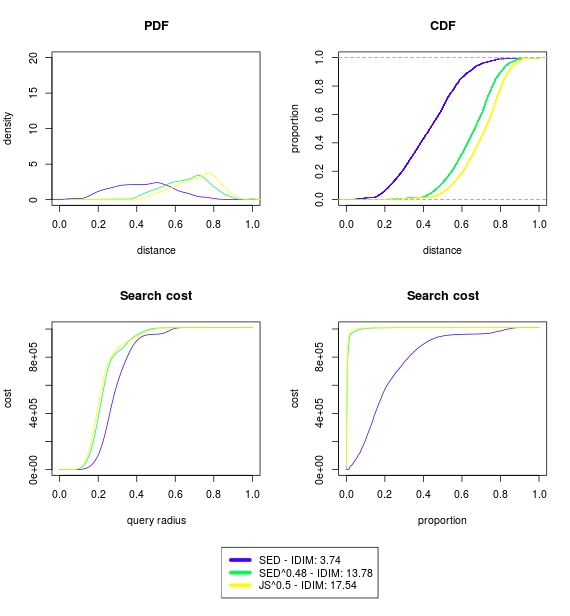
\includegraphics[width=0.9\columnwidth]{gfx/random_trees_cost}
\caption[Metric Search Cost -- Non-uniform Generated Trees]{Generated tree data, showing the predictive costs of searching a metric index from a sample of distance.  Top left is the probability density function, top right is the cumulative density function, bottom left is estimated cost of searching with a particular query radius, and bottom right is the estimated cost of performing a query that is expected to return a given proportion of the data in the index}
\label{fig:random_trees_cost}
\end{figure}

These results again exemplify the benefit of not having to enforce triangle inequality on SED.  Once again, however, there is little to choose between JSD and SED raised to the power 0.48; this time, SED performed slightly better.  This graphical view also demonstrates an important point about this dataset: beyond a very small threshold, raising both metrics to their respective powers had the effect of making searching perform no better than a linear scan. 

Our final dataset was a set of 112,544 color histograms (112-dimensional vectors) from an image database available from SISAP\footnote{http://www.sisap.org}.  Figure \ref{fig:colors_cost} displays the same process as the last dataset.  This time SED was required to have triangle inequality enforced.
\begin{figure}
        \centering
        \subfloat[colors pdf]{
				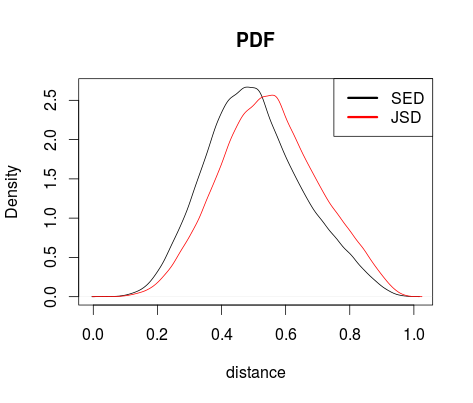
\includegraphics[width=0.35\textwidth]{gfx/cost/colors_pdf.png}
                \label{fig:cost_colors_pdf}
        }%
        ~ 
        \subfloat[colors cdf]{
				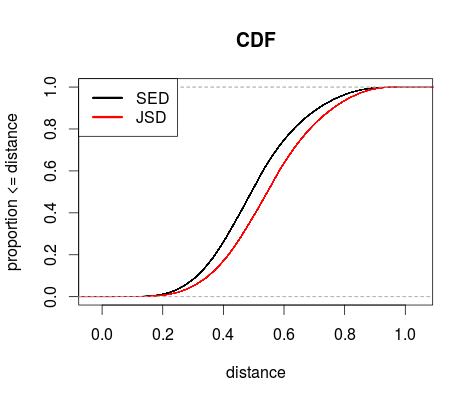
\includegraphics[width=0.35\textwidth]{gfx/cost/colors_cdf.png}
                \label{fig:cost_colors_cdf}
        }
        
         
        \subfloat[colors threshold cost]{
				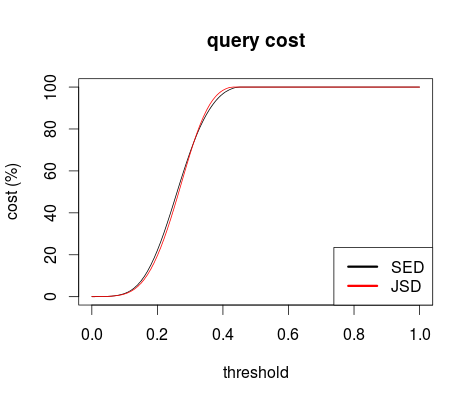
\includegraphics[width=0.35\textwidth]{gfx/cost/colors_threshold_cost.png}
                \label{fig:cost_colors_threshold}
        }
        ~ 
        \subfloat[colors proportion cost]{
				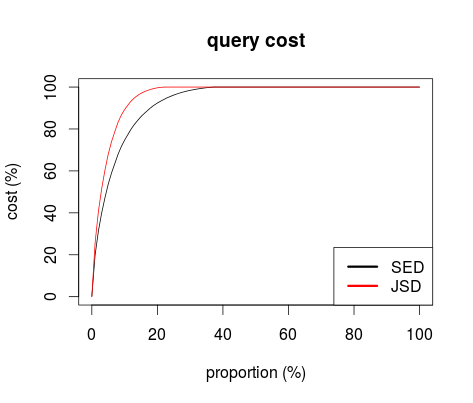
\includegraphics[width=0.35\textwidth]{gfx/cost/colors_proportion_cost.png}
                \label{fig:cost_colors_proportion}
        }
\caption[Metric Search Cost -- Colors dataset]{Colors dataset, showing the predictive costs of searching a metric index from a sample of distance.  Top left is the probability density function, top right is the cumulative density function, bottom left is estimated cost of searching with a particular query radius, and bottom right is the estimated cost of performing a query that is expected to return a given proportion of the data in the index}
\end{figure}
%\begin{figure}[h!]
%\centering
%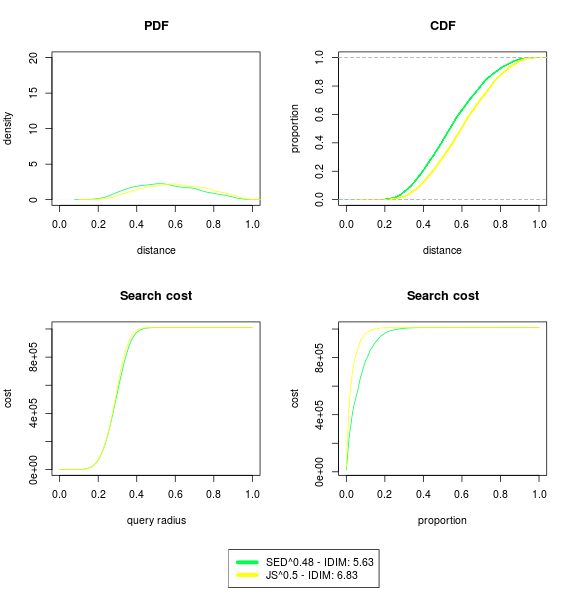
\includegraphics[width=0.9\columnwidth]{gfx/colors_cost}
%\caption[Metric Search Cost -- Colors dataset]{Colors dataset, showing the predictive costs of searching a metric index from a sample of distance.  Top left is the probability density function, top right is the cumulative density function, bottom left is estimated cost of searching with a particular query radius, and bottom right is the estimated cost of performing a query that is expected to return a given proportion of the data in the index}
%\label{fig:colors_cost}
%\end{figure}

In this real-world dataset, there was a clear benefit to using SED over JSD; the cost function grew at a substantially slower rate.  And in general, SED is a better choice for metric search.  This is especially true in the domain of trees, where there is no requirement to enforce triangle inequality, since no violations occur.  Where this requirement does exist SED is at least as good as JSD, and as we have found can even be better.

\begin{figure}
        \centering
        \subfloat[SED]{
				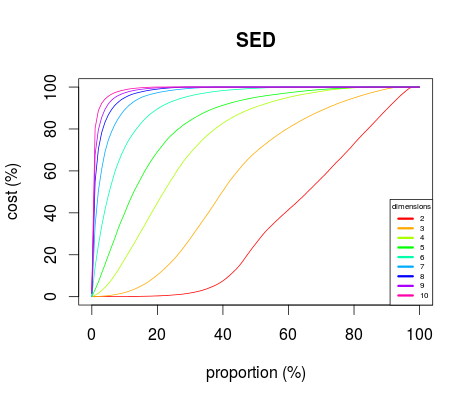
\includegraphics[width=0.5\textwidth]{gfx/cost/shuffled_sed.png}
                \label{fig:shuffled_02}
        }%
        ~ 
        \subfloat[JSD]{
				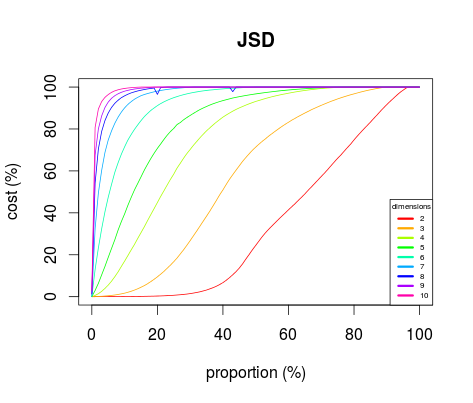
\includegraphics[width=0.5\textwidth]{gfx/cost/shuffled_jsd.png}
                \label{fig:shuffled_04}
        }
\caption[Metric Search Cost -- Generated vectors]{Metric Search Cost -- Generated vectors}
%\label{fig:random_trees_cost}\label{fig:sed_timings_shuffled}
\end{figure}